\newpage
\section{Gecorreleerde subquery’s}

\subsection{Subquery’s in WHERE}

Welke soort subquery mogelijk is, hangt af van de gekozen operator.

$=, >, <, … $	: scalaire (vergelijken met getallen)

Vb:	
\begin{minted}{postgresql}
select spelersnr, naam
from spelers
where spelersnr >
    (select spelersnr 
    from spelers 
    where spelersnr =50) 
\end{minted}
	
IN(…) 		: kolom (vergelijken met kolommen)

Vb: 	
\begin{minted}{postgresql}
select spelersnr, naam
from spelers
where spelersnr IN (
    select spelersnr 
    from spelers 
    where spelersnr >50)
\end{minted}
	
Ze hebben de zelfde output, namelijk alle spelers met een spelersnr boven 50


\subsection{Hoofdquery en subquery}

\bi
\itf Hoofdquery krijgt alles wat in SELECT staat van subquery
\itf Hoofdquery weet niets van detail van subquery, krijgt alleen de output
\itf Subquery weet alles van hoofdquery
\ei

Hoofdquery
Subquery
Vb : 

\begin{minted}{postgresql}

select spelersnr, naam 
from spelers
where spelersnr IN (
    select spelersnr 
    from spelers 
    where spelersnr >50)
	\end{minted}


\subsection{Gecorreleerde subquery}

= subquery waarin een kolom wordt gebruikt die tot een tabel behoort uit een andere select-blok.

\noindent $\Rightarrow$ Subquery kan dus niet autonoom uitgevoerd worden.

Vb: 
\begin{minted}{postgresql}

select spelersnr, naam 
from spelers s 
where spelersnr  IN (
    select spelersnr 
    from boetes b
    where s.spelersnr =b.spelersnr )
\end{minted}

\subsection{Operator EXSISTS and NOT EXSISTS}

\begin{minted}{postgresql}
Select naam 
from spelers s 
where exists (
    select  spelersnr 
    from boetes 
    where spelersnr = s.spelersnr)
\end{minted}

Uitleg :  Elke speler waavoor minstens 1 boete betaald is. Indien er voor 1 speler een rij tevoorschijn komt in de subquery dan zal de where van de hoofdquery true teruggeven.

Voor NOT EXSITS omgekeerd. Zelfde werkwijze.


\subsection{Operator ANY and ALL}

= extra operator, verwacht scalaire waarde en kolomexpressie

\textbf{Voorbeeld all}
Geef van elk team het teamnr en de nr van de speler met het laagste aantal gewonnen sets:

\begin{minted}{postgresql}

SELECT distinct teamnr, spelersnr 
FROM wedstrijden w1
WHERE  gewonnen <= ALL (
    SELECT gewonnen 
    from wedstrijden w2 
    where w1.teamnr  = w2.teamnr)
\end{minted}


\textbf{Voorbeeld any}

Geef de spelersnummers van de spelers voor wie minstens één boete betaald is die groter is dan een boete betaald voor speler 27; deze speler mag zelf niet in het resultaat voorkomen.

\begin{minted}{postgresql}
SELECT DISTINCT spelersnr
FROM spelers inner join boetes b using(spelersnr)
WHERE b.bedrag > ANY(
    SELECT bedrag 
    FROM boetes 
    WHERE spelersnr = 27)
    AND spelersnr <> 27
\end{minted}

Any : Minstens 1

All : allemaal


\subsection{Operator Unique}

\begin{figure}[h!]
\centering
  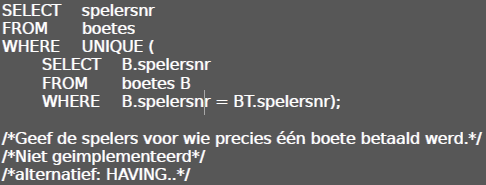
\includegraphics[width=0.5\textwidth]{./figures/unique.png}
  \caption{operator unique}
  \label{fig:operator unique}
\end{figure}

Het spelersnr moet exact  1 keer voorkomen in de subquery. 



\subsection{Operator Overlaps}

\begin{figure}[h!]
\centering
  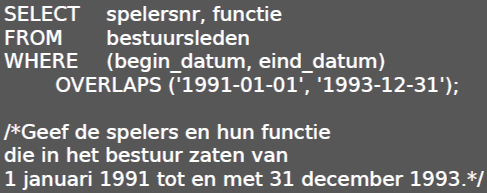
\includegraphics[width=0.5\textwidth]{./figures/overlaps.png}
  \caption{operator overlaps}
  \label{fig:operator ovelaps}
\end{figure}

OVERLAPS :  WHERE (datum1,datum2) OVERLAPS (datumA, datumB)  (de ene periode tussen datum1 en 2 een gemeenschappelijk tijdstip heeft met de andere periode) Indien dit true is worden spelersnr en functie van de betrokken speler getoond.

\newpage
\section{Subqueries examenwiki}
Zie voor meer info naar de slides 03 \_ 1 \_ subqueries (1).pdf

\subsection{Mondeling: Geef de 4 soorten subqueries en leg grondig uit met voorbeelden. }

\begin{enumerate}
    \item Scalaire subgquery
        \begin{enumerate}
   
        \item 1 rij, 1 waarde
        
        \end{enumerate}
        

\item Rij-subquery
\begin{enumerate}
\item 1 rij
\end{enumerate}

\item Kolom-subquery
\begin{enumerate}
\item a.	Elke rij 1 waarde
\end{enumerate}

\item Tabel-subquery
\begin{enumerate}
\item Verzameling rijen en kolommen
\end{enumerate}
\end{enumerate}

\subsection{Scalaire subquery}

\subsection{Rij-subquery}

\subsection{Kolom-subquery}

\subsection{Tabel-subquery}

